\documentclass[a4paper, UTF8]{ctexbook}

\usepackage{amsmath}
\usepackage{amssymb}
\usepackage{amsthm}
\usepackage[dvipdfmx]{geometry}
\usepackage{graphicx}
\usepackage[toc]{multitoc}
\usepackage{paralist}
\usepackage{subcaption}
\usepackage{tabularx}
\usepackage{tcolorbox}
\usepackage{tikz}
\usepackage{wrapfig}
\usepackage{xcolor}
\usepackage[hidelinks]{hyperref}

\def\pgfsysdriver{pgfsys-dvipdfmx.def}
\usetikzlibrary{positioning}

\geometry{a4paper, hmargin=1.25in, vmargin=1in}
\pagestyle{headings}

\makeatletter
\renewcommand\proofname{证明}
\renewenvironment{proof}[1][\proofname]{
	\par
	\pushQED{\qed}
	\normalfont\topsep6\p@\@plus6\p@\labelsep1em\relax
	\trivlist
	\item[\hskip\labelsep\indent\bfseries #1]\ignorespaces
}{
	\popQED\endtrivlist\@endpefalse
}
\makeatother
\newenvironment{desclist}{
	\begin{quote}\begin{compactdesc}
}{
	\end{compactdesc}\end{quote}
}
\newenvironment{enumlist}{
	\begin{quote}\begin{compactenum}
}{
	\end{compactenum}\end{quote}
}
\newenvironment{itemlist}{
	\begin{quote}\begin{compactitem}
}{
	\end{compactitem}\end{quote}
}
\newtheorem{example}{例}[section]

\title{{\Huge 高中数学笔记}}
\author{\textit{Jason Bowen Zheng}}

\begin{document}
\frontmatter
\maketitle
\section*{前言}
简而言之,该数学笔记整理了高中数学的所有知识点,供各位同学参考. 它有点像教科书,但又不是教科书,这一点会在正文中慢慢体现出来.

这本笔记分成了如下部分:

\begin{description}
	\item[代数] 包含方程与不等式、最值值域和恒成立与有解等内容
	\item[函数] 涵盖了函数图像、单调性、对称性、周期性以及导数
	\item[向量和复数] 向量和复数的相关知识
	\item[立体几何] 主要讲述以向量解决立体几何问题
	\item[计数原理] 排列组合和二项式的知识
\end{description}

该数学笔记亦提供了计算器的使用说明,适用于卡西欧\verb|fx-991CN X|.

这本笔记是开源的,您可以在\href{https://github.com/jason-bowen-zheng/math-notes}{这里}获取全部的源代码,亦可以提出改进意见.
\hypersetup{hidelinks}

\begin{flushright}
	\date{2022年11月}于上海
\end{flushright}

\tableofcontents
\clearpage
\mainmatter
\raggedbottom
\chapter{数理分析}
在名为“数理分析”的章节中,您将分别学会解不等式、求代数式的最值值域以及解方程。

\section{不等式}
在初中我们仅仅学了几种不等式的解法,这些很显然是不够的。在这里我们将学习更多的,以及奇奇怪怪的不等式的解法。

\subsection[有名]{有名不等式}
为了方便起见(真的吗?),我们把一些具有明显特征的不等式的集合称为\textbf{有名不等式}。解这些有名不等式必须按照既定的规则去解,否则就不对了。

\subsubsection{一元二次不等式}
如果您去翻一翻教科书,就会发现一元二次不等式的解法好复杂\footnote{这里参照的是沪教版的教科书。}。其实教科书仅仅把可能出现的结果罗列了一遍,并没有简化解法。

那现在重新定义一元二次不等式的解法:对于$ax^2+bx+c>0$且$a>0,\Delta>0$的情况下,大于为一元二次方程的两根之外(如果$x_1<x_2$,则解集为$(-\infty,x_1)\cup(x_2,+\infty)$);小于为两根之间。

\begin{example}
	解不等式$-x^2-5x-4\geq0$
\end{example}
\begin{proof}[解]
	由于二次项系数小于$0$,先变形:\[x^2+5x+4\leq0\]

	后解其对应的方程:\[x^2+5x+4=0\Rightarrow x_1=-4,x_2=-1\]

	转换为不等式的解集:\[x\in[-4,-1]\qedhere\]
\end{proof}

$\Delta\leq0$的情况太麻烦了,我们可以选择画出不等式对应二次函数的图像后再给出解集(无非就是一个解、$\mathbb{R}$或$\emptyset$)。

\subsubsection{分式不等式}
在初中我们也学习了分式方程的解法,千万不要和解分式不等式搞混了。

分式不等式的解法如下:

\begin{enumlist}
	\item 先移项、通分、化标,变为$\frac{x-a}{x-b}\gtrless0$
	\item 可将其看成解$(x-a)(x-b)\gtrless0$的问题
\end{enumlist}

若符号为$\leq$或$\geq$,将分母对应的根由闭变为开。

\subsubsection{绝对值不等式}

\subsubsection{最简指对不等式}
本小节介绍的是\textbf{最简}指对不等式的解法,即解它们的标准形式:\[a^x\gtrless b\text{和}\log_ax\gtrless b\]

\subsection[本质]{用本质解不等式}
在上一小节中我们学习了一些具有明显特征的不等式的解法,这仅仅是一半。接下来我们要面对的是一些奇奇怪怪的不等式。

\section{值域}
顾名思义,值域就是函数因变量(即$y$)的取值范围。

\subsection[本质]{本质(有图)}
一个函数有图像\footnote{一个函数有无图像的标准为是否在第\ref{sec:functionProperty-graphOfFunctions}节介绍过。},画图然后在图上看出值域就行了:

\begin{enumlist}
\item 作图
\item 描深定义域
\item 根据定义域由下往上找到值域的范围
\end{enumlist}

在第\ref{sec:mathsAnalysis-derivative-studyPorpertyOfFunction-figureOfFunction}节中,我们会了解到导数也可以用来求任何函数的值域。

\begin{example}
	求$y=x^2-2x$当$x\in(0,3)$时的值域
\end{example}
\begin{proof}[解]
	先作如图\ref{fig:figure-of-a-function-and-its-domain}的函数图像\footnote{把求值域过程中的函数图像画出来就非常不好看,我们只画这一次。},描深定义域。

	\begin{figure}[htbp]
		\centering
		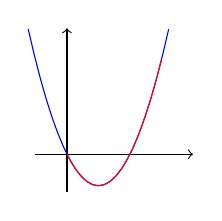
\begin{tikzpicture}[scale=0.4]
			\draw[->] (-1, 0) -- (4, 0);
			\draw[->] (0, -1.2) -- (0, 4);
			\draw[blue, domain=-1.23:3.23] plot(\x, \x * \x - 2 * \x);
			\draw[red, domain=0:3] plot(\x, \x * \x - 2 * \x);
		\end{tikzpicture}
		\caption{画图、描深}
		\label{fig:figure-of-a-function-and-its-domain}
	\end{figure}

	可得其最低点纵坐标为$-1$(是函数的顶点),两端点的纵坐标分别为$0$和$3$,故该函数值域为$[-1,3)$。
\end{proof}

\subsection[复合]{复合(无图)}
但是有些函数的图像你可是画不出来的,比如$y=4^x-2^{x+1}+1$。那就应该使用复合函数求值域的方法了。

如果一个函数$y=f(x)$可复合成$t=g(x)$和$y=f(t)$,那么可先求$g(x)$的值域,记为$A$。然后以$A$为定义域求$f(t)$的值域
(其中$f$、$g$均可作图)。

\subsubsection{根式复合}
\subsubsection{分式复合}

\subsection{非复合}
上面介绍了这么多的复合函数求值域的方法,虽然多,但不可能用在所有函数上。那这些无法复合函数我们就不能求出它们的值域。

但是我们非常的幸运,拿到了一个单调函数(或者说函数在定义域内单调),那还是有办法的,直接代端点就可以了。

\begin{example}
	求$y=(\frac{1}{2})^x+(\frac{1}{3})^x$当$x\in(-\infty,2]$时的值域
\end{example}
\begin{proof}[解]
	由题意得,函数单调递减。

	$\therefore y\in[\frac{13}{36},+\infty)$
\end{proof}

\section{基本不等式}
与值域不同,基本不等式只能用来求代数式的最值,而且有些许的限制。

基本不等式是由以下三个不等式组成的:
\[a^2+b^2\geq2ab\]
\[a+b\geq2\sqrt{ab}\]
\[2(a^2+b^2)\geq(a+b)^2\]
它们等号成立的条件都是$a=b$。

\chapter{立体几何}
我们在初中时期学习了平面几何,研究了平面上一些简单图形及其几何性质;在高中时期,我们也通过三角比及三角函数对三角形有了更深入的理解。现在,我们将增加一个纬度,研究三维空间中的几何体的性质。与其它高中的知识相比较,甚至是与初中的平面几何比较,立体几何都是简单的:它更注重于计算,而非证明,也不需要苦思冥想如何添辅助线。那么,放松,进入立体几何的世界吧!

\chapter{立体几何}
我们在初中时期学习了平面几何,研究了平面上一些简单图形及其几何性质;在高中时期,我们也通过三角比及三角函数对三角形有了更深入的理解。现在,我们将增加一个纬度,研究三维空间中的几何体的性质。与其它高中的知识相比较,甚至是与初中的平面几何比较,立体几何都是简单的:它更注重于计算,而非证明,也不需要苦思冥想如何添辅助线。那么,放松,进入立体几何的世界吧!

\end{document}
